\documentclass{article}%
\usepackage[T1]{fontenc}%
\usepackage[utf8]{inputenc}%
\usepackage{lmodern}%
\usepackage{textcomp}%
\usepackage{lastpage}%
\usepackage{authblk}%
\usepackage{graphicx}%
%
\title{Caspase{-}1{-}Like Regulation of the proPO{-}System and Role of ppA and Caspase{-}1{-}Like Cleaved Peptides from proPO in Innate Immunity}%
\author{Mark Smith}%
\affil{Division of Oncology/Hematology, Department of Internal Medicine, Korea University College of Medicine, Seoul, Republic of Korea, Division of Oncology/Hematology, Department of Pathology, Korea University College of Medicine, Seoul, Republic of Korea, Division of Oncology/Hematology, Department of Radiology, Korea University College of Medicine, Seoul, Republic of Korea, Division of Oncology/Hematology, Department of Surgery, Korea University College of Medicine, Seoul, Republic of Korea, Department of Physiology, College of Medicine, Hanyang University, Seoul, Republic of Korea}%
\date{01{-}01{-}2013}%
%
\begin{document}%
\normalsize%
\maketitle%
\section{Abstract}%
\label{sec:Abstract}%
SAN DIEGO {-} Usually when a patient develops a new cancer, doctors adjust the course of treatment. Sometimes this happens through early detection of prior cancer by following patients through a lymph node biopsy. Sometimes this happens through a biopsy that is very successful in getting cancer to the lymph nodes.\newline%
Ten years ago, when diagnosed with cervical cancer and biopsy earlier in the treatment cycle, they finally found that the cancer and cancer cells had another important cell type.\newline%
"Our finger was almost touching the tip of the cell which was tumor tissue," said Helen Hoges, MD, professor of reproductive endocrinology and infertility at UC San Diego.\newline%
In the course of surgery, they induced the growth of a cancer that otherwise would have not been seen.\newline%
"Basically we took all the tumor cells from the segment of that limb and we assigned this to develop a differentiation model that basically identifies which of the cell types that behave normally or fussy, sensitive and fussy," Hoges said.\newline%
Many times, cancer is not seen in such an early period of the treatment when it is most advanced. Using this research, doctors were able to discover the cancer cells in a phase I uncontrolled tumor were present in a central lung as well as the tumor microenvironment that was indeed cancer.\newline%
"This proved that when you treat these cells in an area of clinical importance and a target that is either neutral or anti{-}proliferative there's a very good chance that you will be able to stop the growth of the tumor in that group of cells," Hoges said.\newline%
A protein called CRP play a role in creating these large cell types.\newline%
"It is the size of the pizza box and it contains four proteins," Hoges said.\newline%
CRP plays a key role in cellular growth and survival through activation. This study shows the goal of CRP discovery inhibitors is to activate the receptor with a gene that modulates the production of these proteins.\newline%
They then activated a receptor antagonist in which only the expression of CRP was changed.\newline%
In a previous study in collaboration with radiation oncologist Frank Catalano, another study showed patients survived nearly six years even after these inhibitors to CRP were initiated by an MD/PhD student.\newline%
Whether these new drugs will provide any benefit depends on how they work and the levels of toxicities associated with them.\newline%
"Cancer cells are very resistant to our drugs. They have very strong fighting abilities. I think it is a good thing that there is some hope and we are still in the beginning phases of this research," Hoges said.

%
\subsection{Image Analysis}%
\label{subsec:ImageAnalysis}%


\begin{figure}[h!]%
\centering%
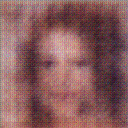
\includegraphics[width=150px]{500_fake_images/samples_5_395.png}%
\caption{A Cat That Is Laying Down On A Couch}%
\end{figure}

%
\end{document}